\subsection{Overview}
An essential part of the platform design is to satisfy not only functional requirements but non-functional requirements as well.This means that architectural choices are crucial at this point of the development for the sake of achieving the desired output in terms of requirements ,performance ,scalability and user experience.\\
An important focus will be set on how the different systems interact with each other and the back-end to obtain the events as required by sec. 3 of the RASD.Furthermore choices regarding up scaling and redundancy will be discussed.\\

%----------------%
% COMPONENT VIEW %
%----------------%
\subsection{Component View}
This section focuses on the component overview giving an insight on their core functionality and various interfaces.For more detailed information about component interfaces see \hyperref[sec:CInter]{\emph{section 2.5}} \\
A first classification of components can be made at a high level:
\begin{itemize}
\item \textbf{\hyperref[sec:Server]Server} provides the core functionality of the platform. The server incorporates the biggest part of the \emph{business logic} and stores some \emph{data} locally.
\item \textbf{\hyperref[sec:UserClient]User Client} provides a high level representation of the real user clients. It is considered a \emph{thin client} as it leaves most of the functionalities to the Server.
\item \textbf{\hyperref[sec:OnBClient]On-Board Client} provides navigation functionalities done exclusively client-side , whilst other functionalities are left to the server side (like  authentication).
\end{itemize}
As mentioned above the platform is designed using the \emph{client-server}paradigm. Component interactions are handled by the server which is able to receive calls from the clients . Client interaction is never done peer to peer but via server.


\subsubsection{Server}
The server is composed of :\\[0.4in]
\textbf{Back-End Application}\\[0.1in]
The Back-End Application is the  component that handles most of the business logic.
The application is written in Java EE and to fulfil its tasks (see section
3 of the RASD) it needs to interface with the Internet network using
the HTTPS protocol and the JAVA API for RESTful Web Service, with a
MySQL database and GooleMaps API.\\[0.4in]
\textbf{Back-End internal components}\\[0.1in]
\begin{itemize}

\item \textbf{User manager}\\
This component handles user data, registration and authentication.The user manager has direct access to the DBMS and receives read and write requests from the RESTful API.

\item \textbf{Notification manager}\\
This component is responsible for implementing the push notification service towards
the user-side applications.
It is necessary to have this type of module running in the back-end because
there are cases in which a communication must happen between the clients and
the back-end, but no direct request is made to the RESTful API by the clients:
for example when the reserved car is nearby, the system must send the user a 'ready to unlock' notification.

\item \textbf{Vehicle manager}\\
The car manager component's job is to manage all the vehicles throughout the city.It can access the DBMS to query vehicle information but stores essential vehicle information locally such as location ,battery level and number of seats.Car positions
are managed through the Position manager.

\item \textbf{Position manager}\\
Keeps track of car positions around the city. When the Search manager gets triggered it forwards requests to the Position manager to get all available cars in compliance to the user input. It updates car positions through the vehicle manager at the end of each ride through the Vehicle manager. Moreover it handles the fair car distribution scenario when triggered by the on-board display. 

\item \textbf{Search manager}\\
The search manager component handles all incoming search requests forwarded by the user applications and interfaced through the RESTful API. The main functionality is to handle the user input and query the vehicle manager accordingly, returning the desired output to the user.\\In the event of a booking request the search manager forwards the demand to the Ride Manager.

\item \textbf{Ride manager}\\
The Ride manager component examines all incoming reservation request and creates \textit{Ride objects} according to the user selection and user data.The ride manager
is connected to the following components:
\begin{itemize}
\item \textit{Vehicle manager}: need to communicate and receive communications about car status changes in terms of availability, battery level and location.
\item \textit{Notification manager}: need to inform the user about remaining time to unlock the car or send the user 'ready to unlock ' notifications. Moreover it sends messages to the on-board display to inform the user about the response to a \textit{end ride request}.\\[0.4in] 
\end{itemize}
 
\end{itemize}

\textbf{Data Base}\\[0.1in]
The MySQL database fulfills the task of storing and granting access to all
the data generated and used by the service.\\
The connection between the Java EE application and the Data Base is supported
by the \emph{JDBC connector} \footnote{\url{http://dev.mysql.com/downloads/connector/j/}}.For more information about the data base see \hyperref[sec:DMV]{\emph{section 2.7}}.


\subsubsection{User Client}

As stated in section 2.4.2 of the RASD a native mobile application is developed
for Android, iOS and Windows Phone as well as Web application for the main browsers.
To fulfil the requirements expressed in section 3 of the
RASD, all the clients need to communicate with the Server making calls to
the REST API using platform specific API for REST HTTP calls.

\subsubsection{On-Board Client}
The on-board client needs to provide navigation functionality without interacting with the PowerEnjoy Server but directly through GoogleMaps API. At the beginning of each ride an authentication via PinCode is requested and verified server side.\\Safe Areas are stored locally on the client and updated only when the changes on the DB occur.On the other hand charging stations need to be updated in real-time as it can happen that charging stations are currently out of capacity.
\clearpage


\FloatBarrier
\begin{figure}
\subsubsection{Diagrams}
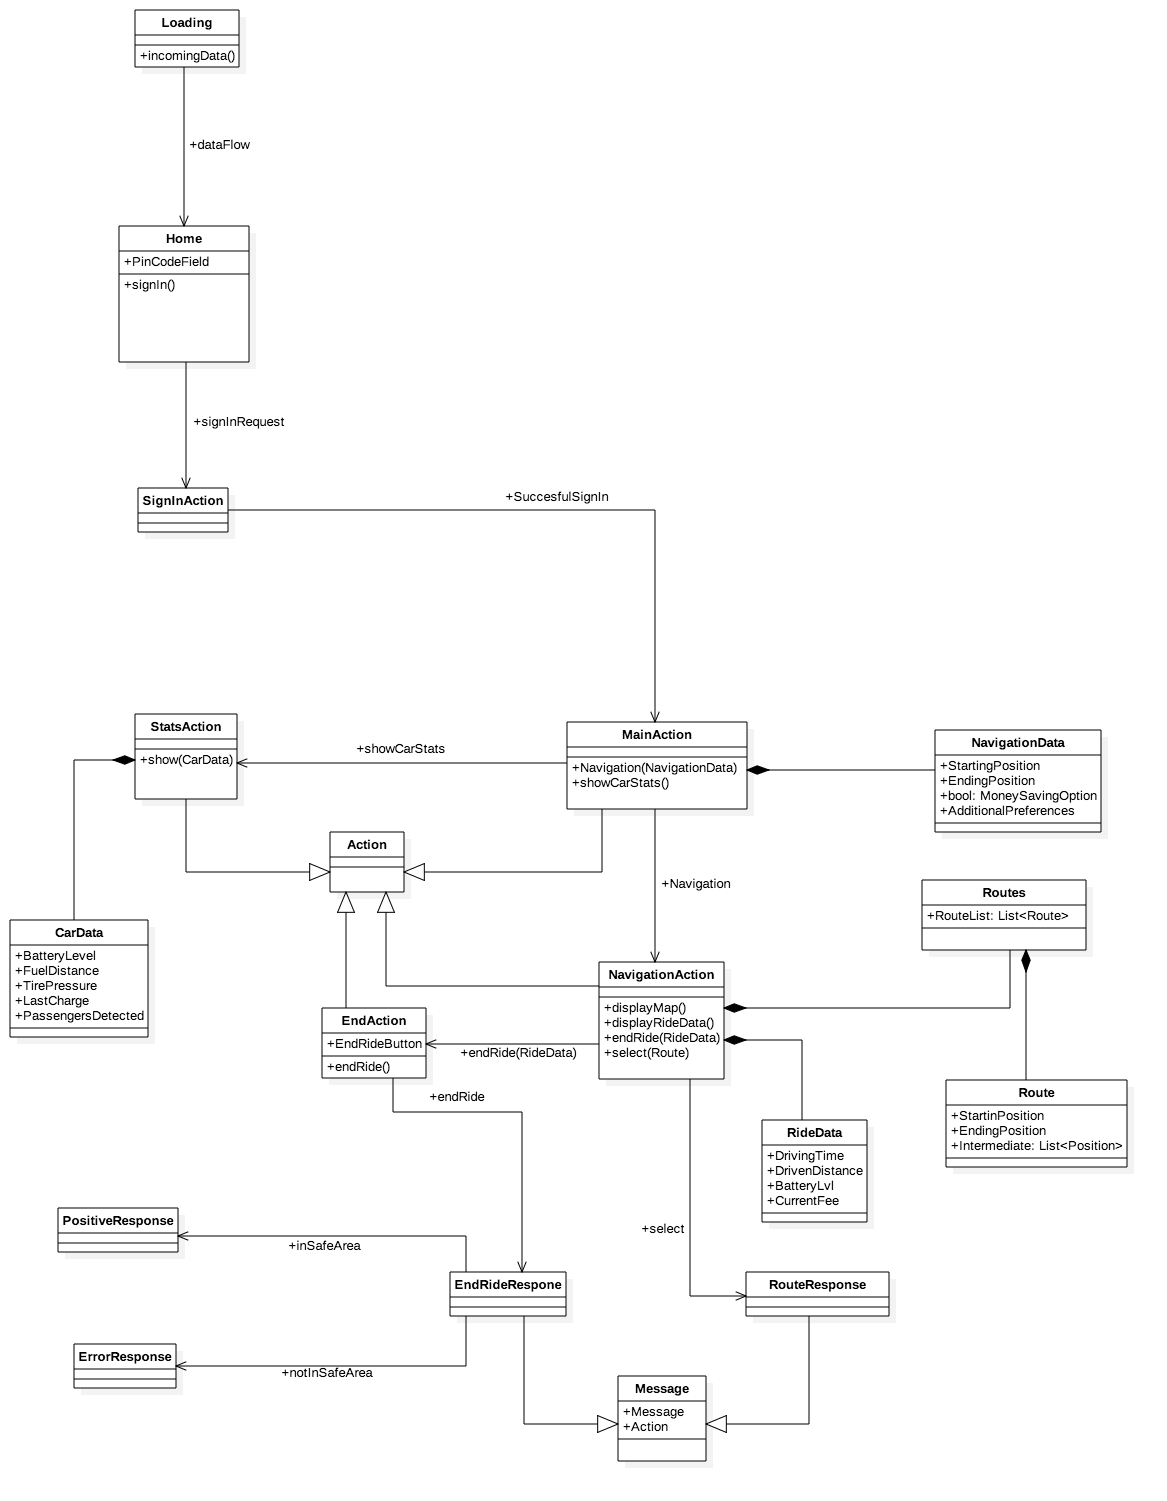
\includegraphics[scale=0.35]{Images/ClassDiagram/User.png}
\caption{User Application Class Diagram}
\end{figure}
\FloatBarrier

\FloatBarrier
\begin{figure}
\hspace{-15mm}
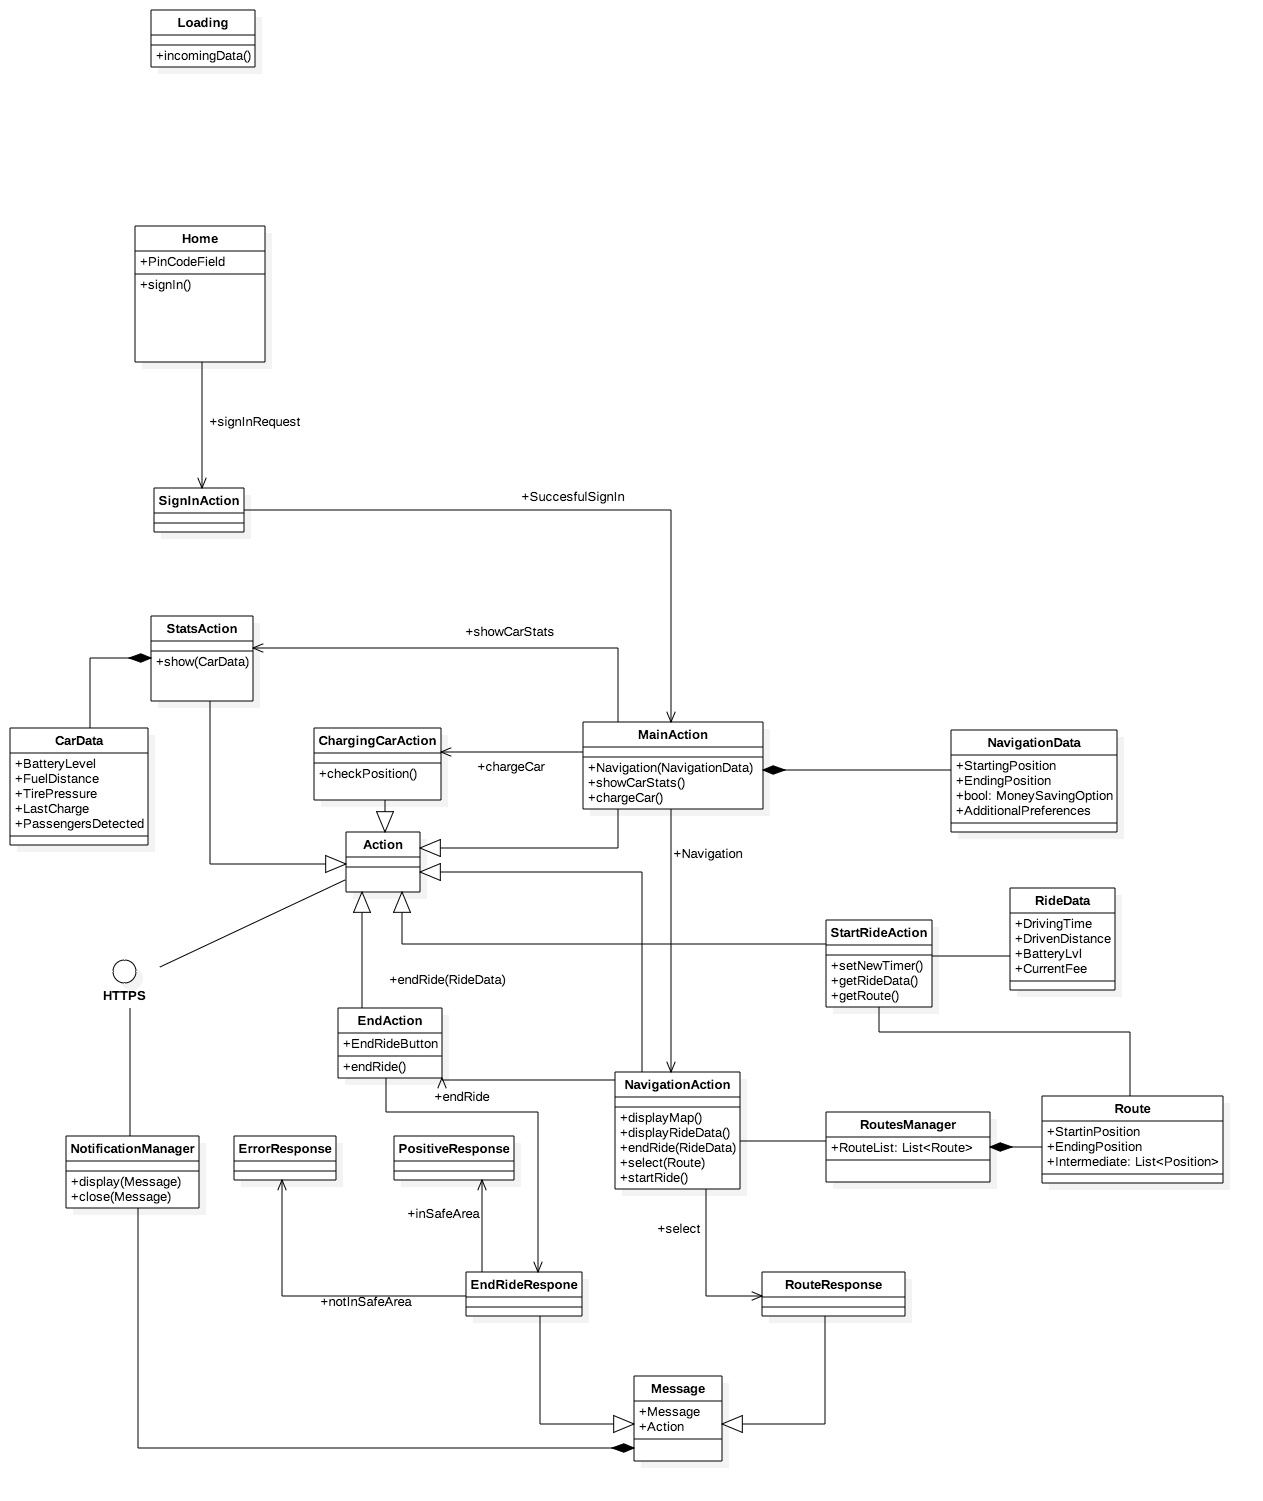
\includegraphics[scale=0.35]{Images/ClassDiagram/Display.png}
\caption{On-board Class Diagram}
\end{figure}
\FloatBarrier


\FloatBarrier
\begin{sidewaysfigure}
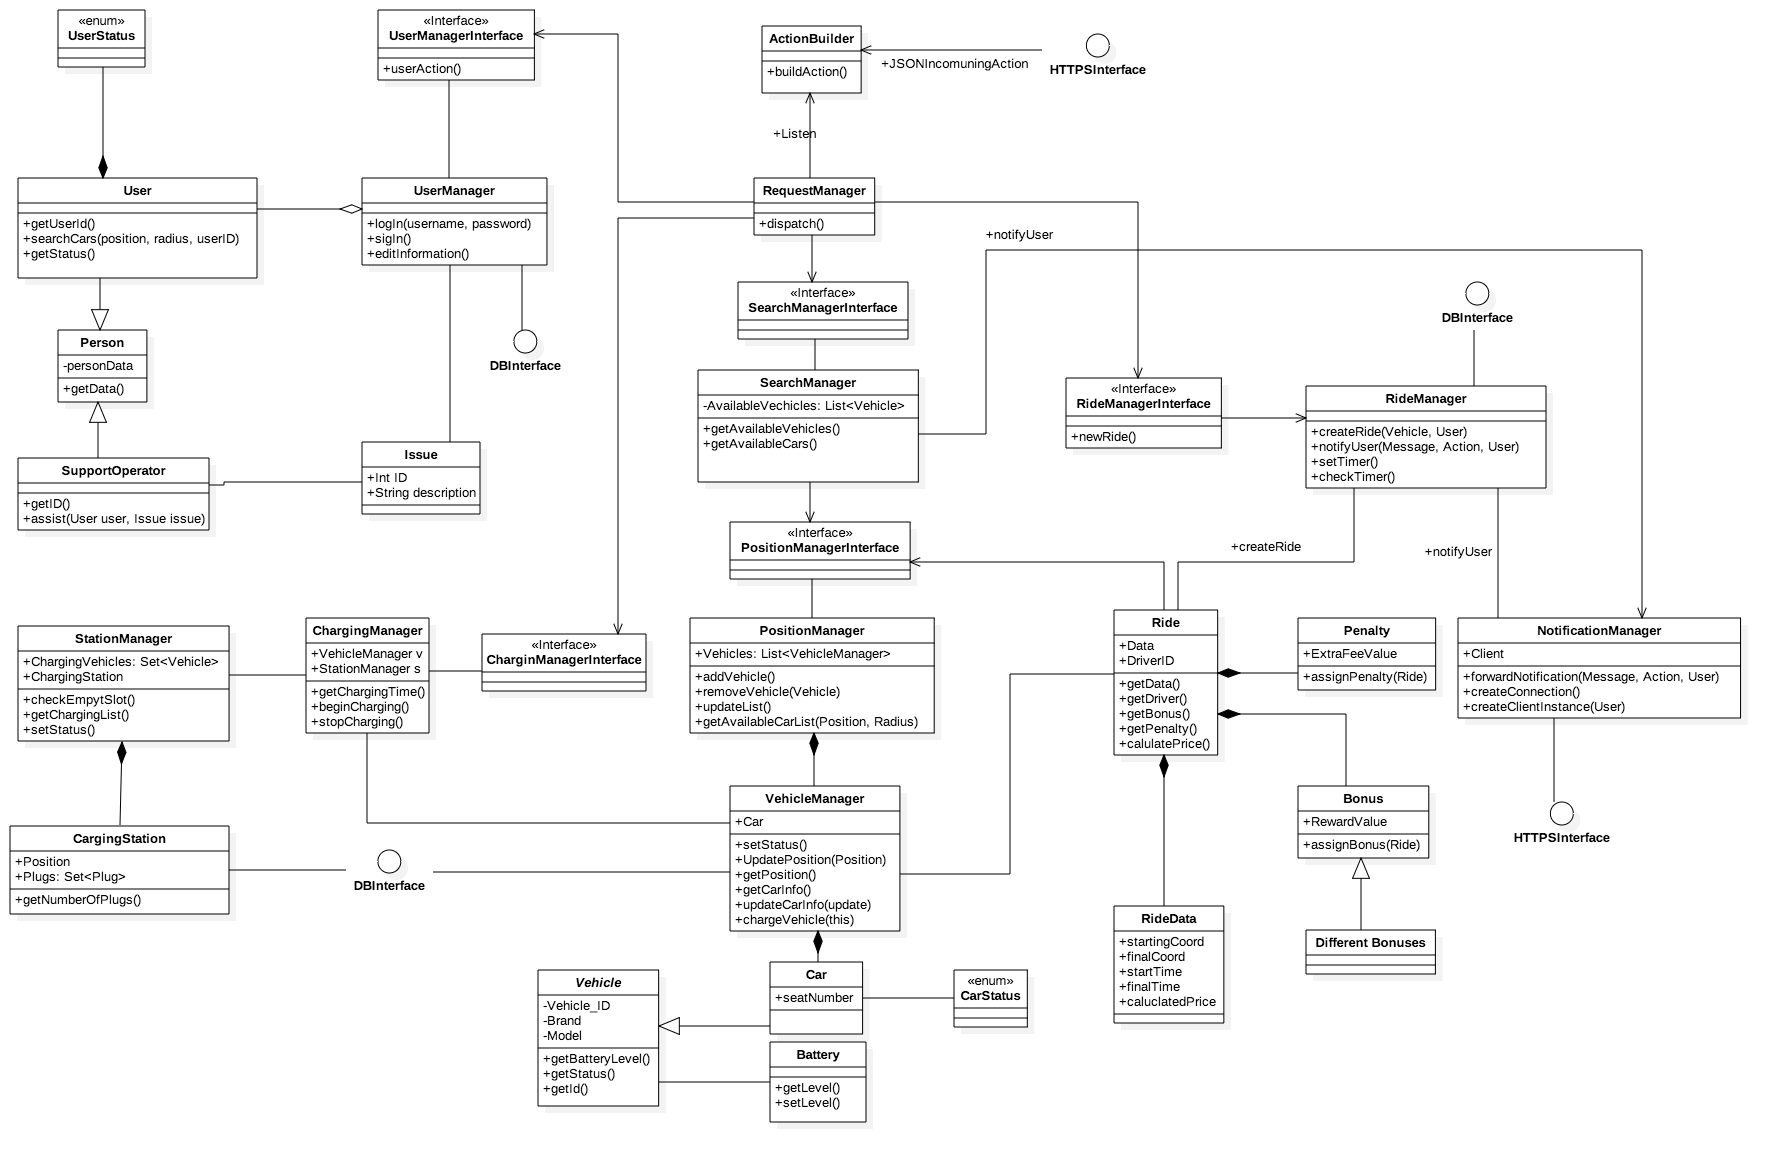
\includegraphics[scale=0.35]{Images/ClassDiagram/BackEnd2.png}
\caption{Back-End Class Diagram}
\end{sidewaysfigure}
\FloatBarrier
\newpage

\subsection{Deployment View}
\label{deploy}
The following section contains a schema of the hardware infrastructure.
It was decided to omit the representation of the purely network-related hardware (routers, switches, etc.).
The chosen architecture is a typical web-based client-server architecture,
with the following components:
\begin{enumerate}
\item \textbf{Primary and BackUp Storage}: the Primary DB is a long term storage system on which the operational database is saved. This node provides the highest Read/Write speeds and is used in normal operational regime.The BackUP DB is a long term storage system with high reliability property. It is mainly used to store data backups and becomes fully operational in the event of total failure of the Primary RDBMS or DBMS nodes.
\item \textbf{Primary RDBMS Server}: server dedicated to run the DBMS software on account of the main server  and to manage the communication with the secondary storage node. This node is connected to the main server, from which it receives requests, and the storage nodes (either primary or secondary - the connection is transparent to the node and is hot-swappable in the event of a failure).
\item \textbf{Secondary RDBMS Server}:server dedicated to run the DBMS software and
manage the backup requests from the primary DBMS server. The node is connected to the secondary storage and to the primary DBMS server, for the reasons described above.
\item \textbf{Main Server}: a typical rack of servers dedicated to run the main back-end application.The rack is composed by independent nodes managed by usual
load balancing technology and is able to be fully functional under average load of the system.The redundancy of the rack has the dual function of improving fault tolerance and performance under above-average load conditions.\\
\end{enumerate}

\FloatBarrier
\begin{figure}
\centering
\hspace{-5mm}
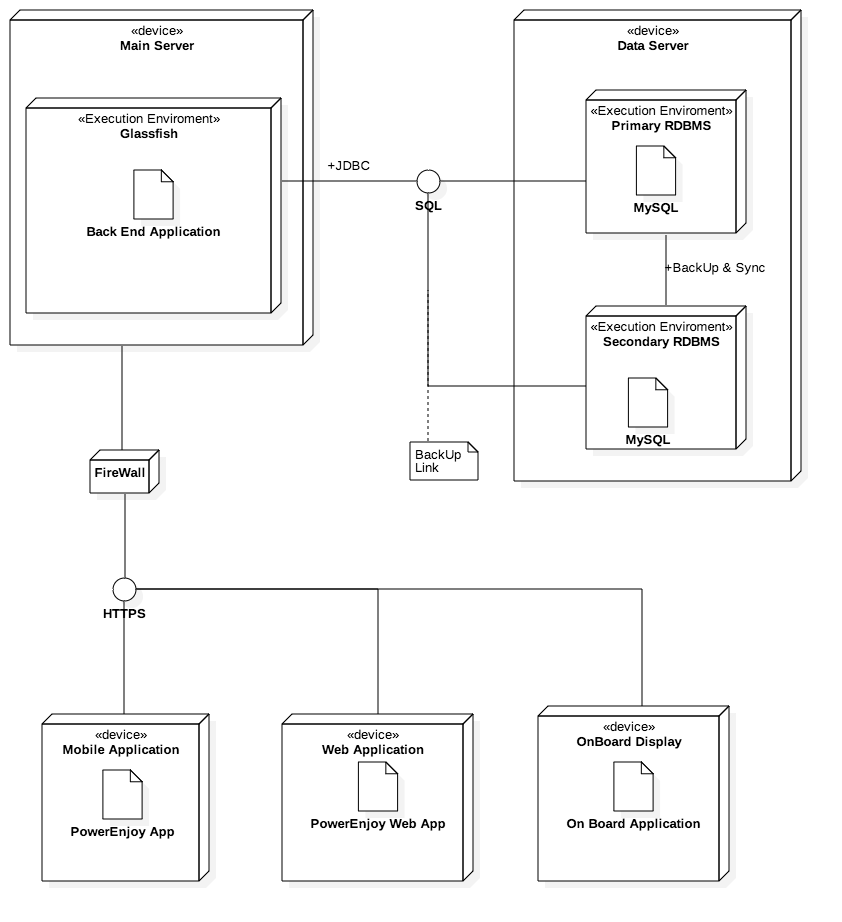
\includegraphics[scale=0.38]{Images/DeployDiagram/Deploy3.png}
\caption{Deployment Diagram}
\end{figure}
\FloatBarrier

%---------------------
% RUNTIME VIEW
%---------------------

\subsection{Runtime View}
\subsubsection{Server View}
This section focuses on the Runtime View of the system.
While the system is up and running, the \emph{Server} receives many \emph{HTTP requests}
from different clients that are handled by a \emph{Load Balancing} component that
distributes the calls evenly to every real machine client.
Every search request is not stored in the DB but is stored locally for processing purposes. Ride request on the other hand are stored on the MySQL databases as it is necessary to keep track of user rides. 
From the internal point of view of the Back-End application, user requests (search, ride or data request) are at first parsed by the Request Manager and the dispatched to Java object that is in charge of computing the result of that request.
\subsubsection{Client View}
From the client point of view, when a User opens his application, the client starts a first "handshake" to check for basic authentication data and if it's successful, the client can proceed with requests.
The flow of a request start from a User Interface component (like a button) and is finally handled by the class that implements the HTTP interface.\\
When a User enters a car a similar process is used but a User pin code has to be entered for authentication purposes.\\
\newpage
\FloatBarrier
\begin{figure}
\subsubsection{Diagrams}
\centering
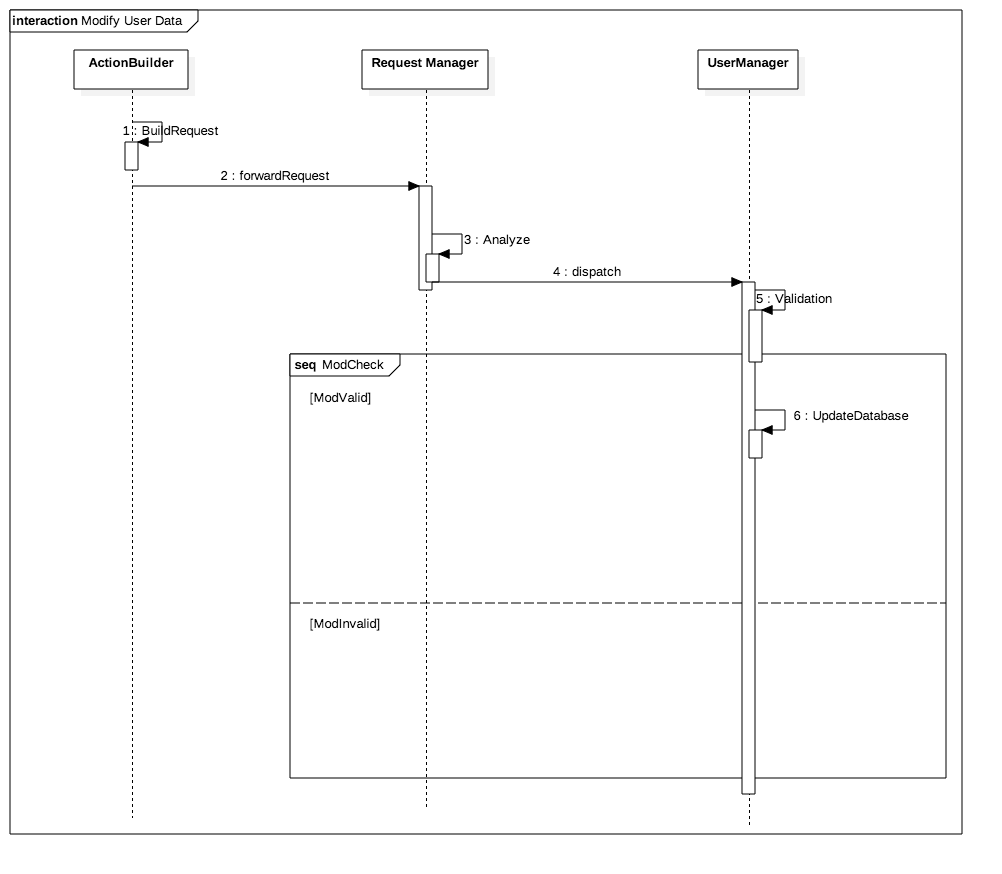
\includegraphics[scale=0.4]{Images/Sequence/seq1.png}
\caption{Data modification sequence diagram}
\end{figure}
\FloatBarrier
\clearpage
\FloatBarrier
\begin{figure}
\centering
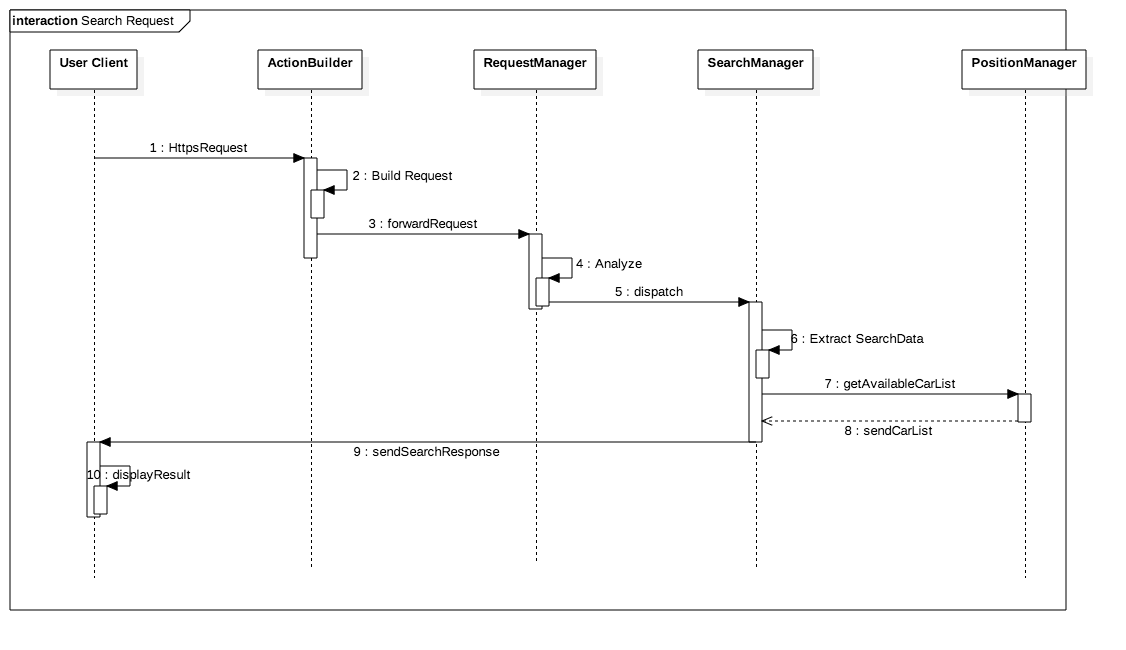
\includegraphics[scale=0.4]{Images/Sequence/seq2.png}
\caption{Search action sequence diagram}
\end{figure}
\FloatBarrier
\clearpage
\FloatBarrier
\begin{sidewaysfigure}
\centering
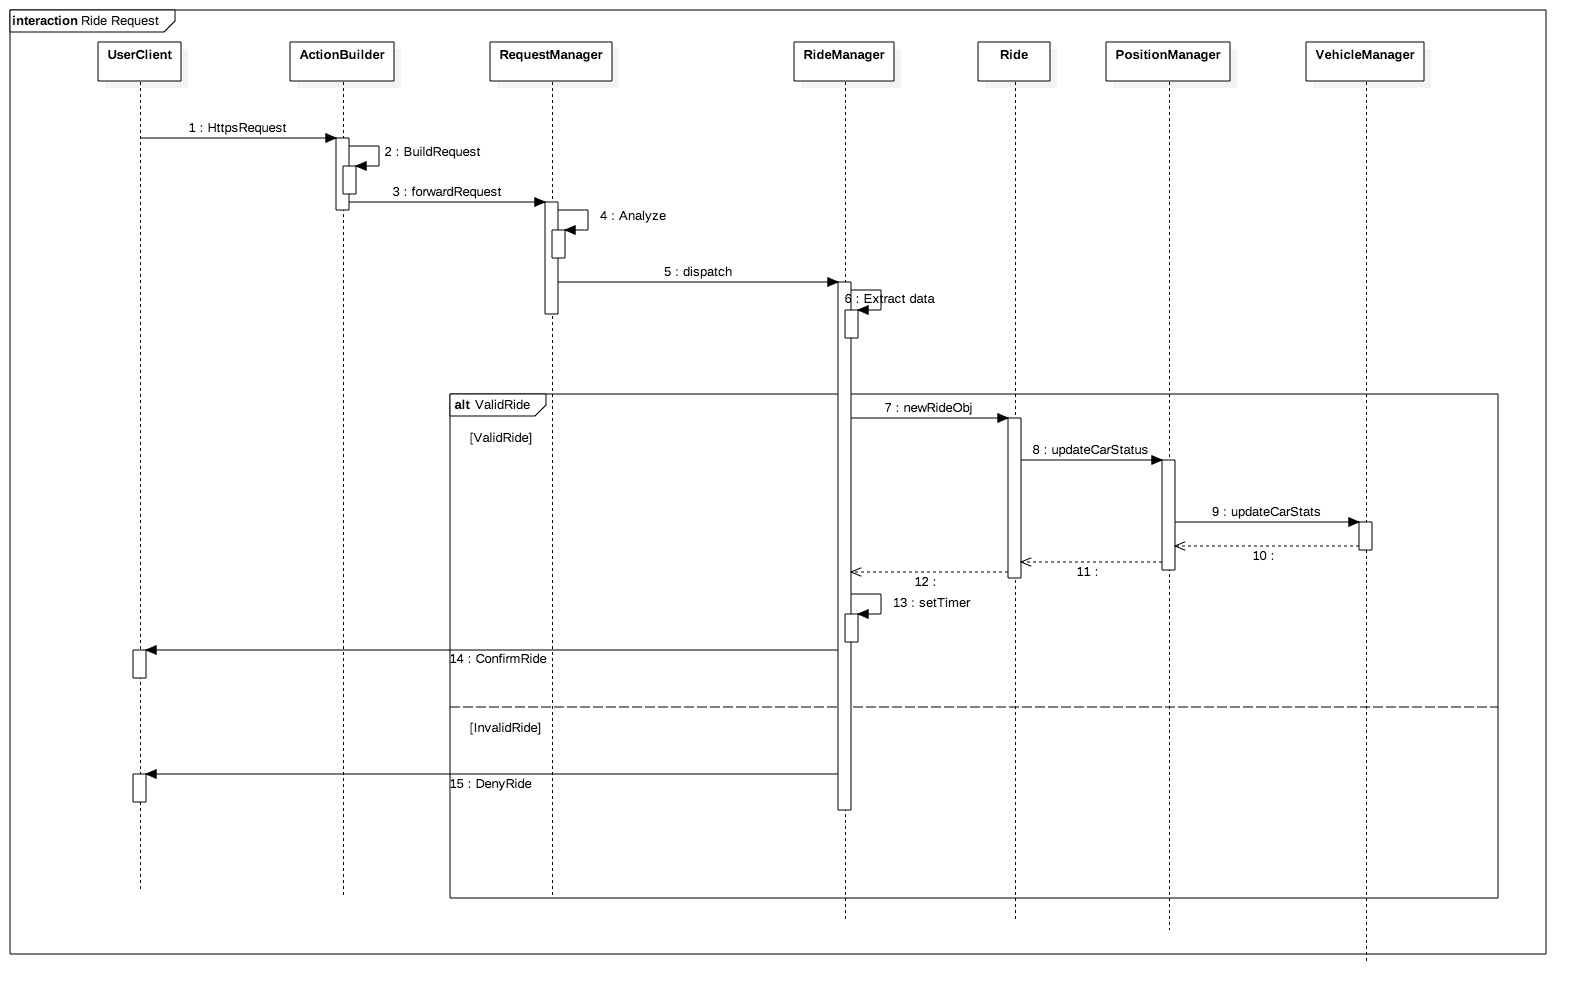
\includegraphics[scale=0.4]{Images/Sequence/seq3.png}
\caption{Search action sequence diagram}
\end{sidewaysfigure}
\FloatBarrier
\FloatBarrier
\begin{sidewaysfigure}
\centering
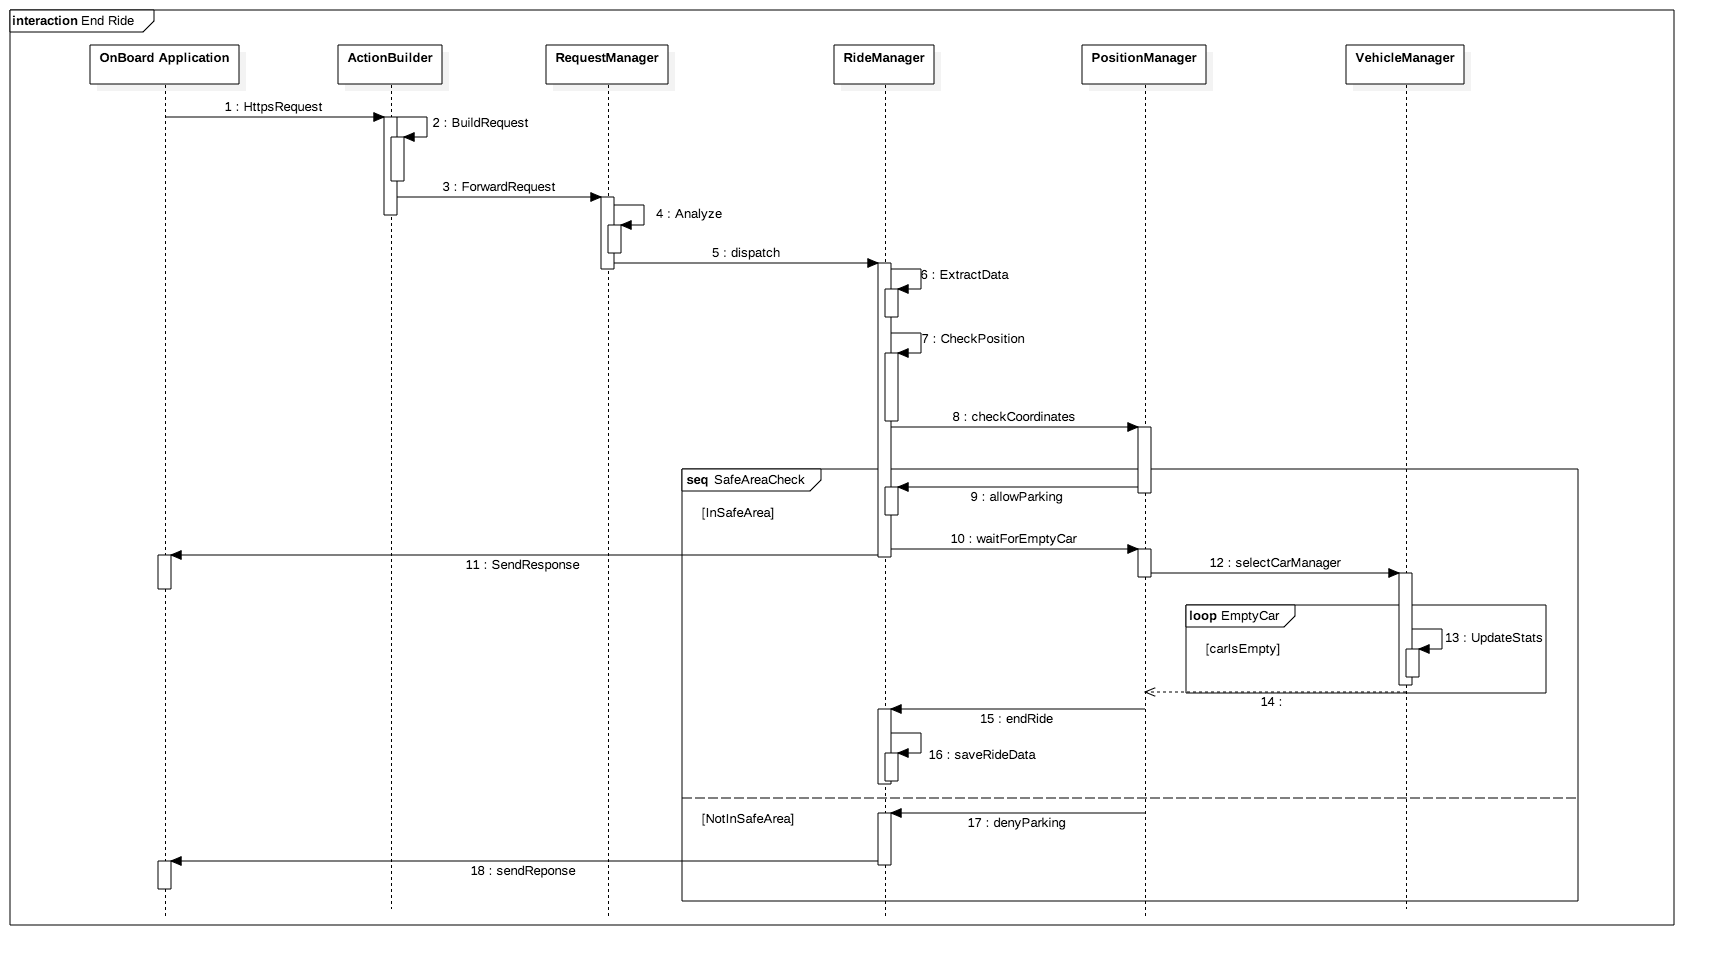
\includegraphics[scale=0.4]{Images/Sequence/Seq4.png}
\caption{Search action sequence diagram}
\end{sidewaysfigure}
\FloatBarrier




\newpage



%---------------------
% COMPONENT INTERFACES
%---------------------

\subsection{Component Interfaces}
\label{sec:CInter}
This section provides a description of the interfaces between the main components
of the system.
\\[0.2in]
\textbf{Server interaction}\\
\begin{itemize}
\item \textbf{Back-End application $\rightarrow$ Database}\\
The \emph{back-end application} uses SQL language to query the \emph{database}. Queries from Java 
are supported by the \emph{Java Database Connectivity (JDBC) API} \footnote{\url{http://www.oracle.com/technetwork/java/javase/jdbc/index.html}}.JDBC comes extremely handy thanks to it powerful \emph{"Write once, Run Everywhere "}feature.
\item \textbf{Back-End$\rightarrow$ Client Application}\\
The connection between the \emph{Back-End} and the \emph{Client application} is managed by the internet network based on a HTTPS protocol and supported by the RESTful API service.To add further security to the data flow an intermediate Firewall is deployed.
\item \textbf{Back-End $\rightarrow$ On-Board Application}\\
The connection between the \emph{Back-End} and the \emph{On-board application} is managed by the internet network based on a HTTPS protocol and supported by the RESTful API service.To add further security to the data flow an intermediate Firewall is deployed.
\end{itemize}
\textbf{RESTful API}\\The RESTful API is a gateway communicator between clients and the back-end system: it's a stateless service which provides methods for data submission or requests returning the requested computations as a result.\\
RESTful API are an optimal solution for an application that must handle a vast number of users on a different number of platforms as it allows to guarantee the same user experience on all platforms. Furthermore the architectural properties positively affected by the constraints of the REST architectural include many important quality requirements such as performance, scalability and reliability.\\[0.2in]
\textbf{JDBC}\\
JDBC is a Java API that manages the access of a generic client to a database. In
our platform, it acts as interface between the \emph{back-end application} and the
DBMS component (on both the primary and secondary nodes).
\subsection{Selected architectural styles and patterns}
This section highlights both hardware and software selected styles and design
patterns.The following patterns are meant to be guidelines for developers and may not reflect entirely the actual pattern adopted as different choices can be made during development phase.\\
\subsubsection{Software patterns}
The overall software system must follow the \emph{Object Oriented Paradigm}.
In particular, developers should follow the principles of \emph{encapsulation, composition, inheritance, delegation and polymorphism}.\\
Developers should promote code reuse and should try to solve programming
problems using common OO Design Patterns\footnote{\emph{Design Patterns: Elements of Reusable Object-Oriented Software by Erich
Gamma, Richard Helm, Ralph Johnson, John Vlissides}}
Code produced by developers, must be fully commented and documented in
order to promote simple refactoring and maintenance.\\
Some patterns used in the description of the architecture are considered essential:
\begin{itemize}
\item \textbf{Publish/Subscribe}:The publish/subscribe design pattern is used to interface the Ride Manager with the Notification manager, where the latter is the
subscriber and must react to events suitably generated by the former, which is
the publisher.
\item \textbf{Push}: Push technology is an implementation of the publish/subscribe design pattern, which is widely used in modern mobile applications to manage notification services.\\
In our platform, requests are generated by the Notification manager and
picked up by the user-side mobile applications, which react to them by displaying
the suitable notifications on the users’ devices.
\end{itemize}
\subsubsection{Hardware patterns}
As outlined in the \emph{deployment view} \ref{deploy} the platform is obviously designed as a client-server architecture, in which the back-end nodes are the server and the various users' devices are the clients.\\
The system is based on a \emph{three tier architecture}:
\begin{itemize}
\item \textbf{First Tier}: composed of client devices (user application and on-board application).
\item \textbf{Second Tier}:composed of a rack of servers.
\item \textbf{Third Tier}: composed of database servers controlled by load balancing and storage units.
\end{itemize}
We chose to deploy each logical layer on a physical tier :
\begin{itemize}
\item \textbf{Presentation Layer}: is the layer responsible for displaying data to
the users and for transmitting input data to the business logic layer.\\
The presentation layer is deployed in the First Tier.
\item \textbf{Logic Layer}:This layer is responsible for receiving data
from the presentation layer, for computing and transmitting a response(using also data provided by the data store layer) to the presentation
layer.This layer implements most of the business logic and is deployed in the
second tier.
\item \textbf{Data Storage Layer}:This layer is responsible for storing all the data meaningful to the system. This layer is deployed in the third tier.
\end{itemize}

\newpage

%----------------%
% DATA VIEW      %
%----------------%
\subsection{Data Management view}
\label{sec:DMV}
This section focuses on how the data is stored and structured.
\subsubsection{Storing policy}
Data storage about people or physical belongings to PowerEnjoy are never automatically eliminated from the DB. On the other hand \emph{Rides} older than 2 years are automatically eliminated from the DB to save storage space and 
speed up search queries.\\
In order to reduce the load on the Server and to speed up user’s query
response, all the data that does not change frequently (like the user’s profile
data) is saved locally on the device and reloaded only when a modification
of the profile occurs.

\subsubsection{Entity-Relation Diagram}
\begin{center}
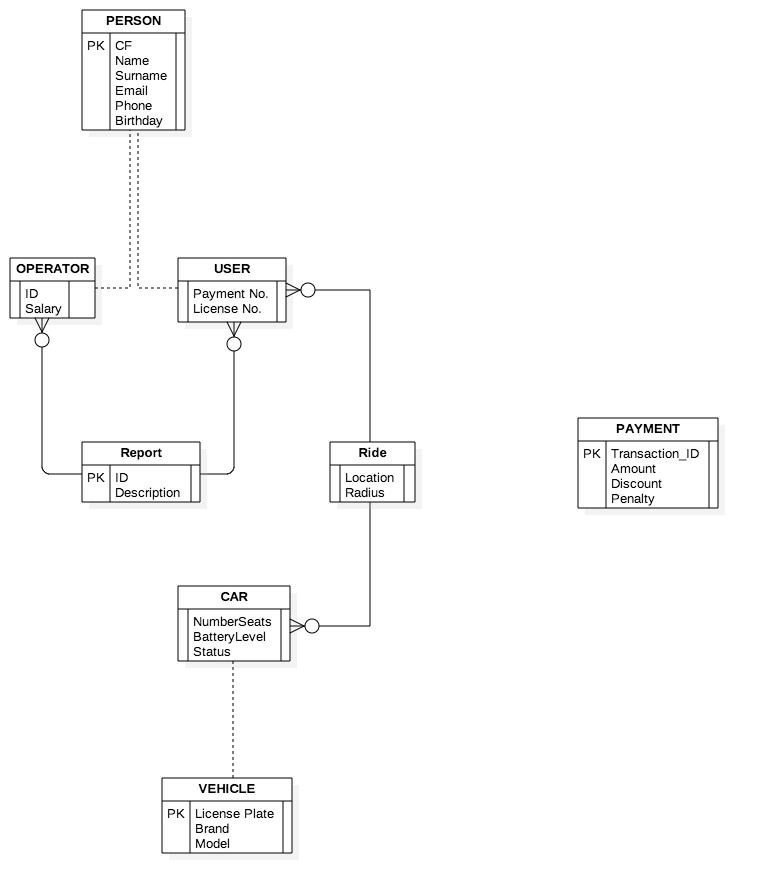
\includegraphics[scale=0.35]{Images/ER/ER.png}
\end{center}
The above shown figure represents the structure of the database. For better readability only vital entities are represented while others (like employees or managers) are omitted.
\begin{itemize}
\item \textit{Person}: is the generalisation of the operator and user entities. 
It holds common information and is identified by a \emph{Codice Fisicale}. All attributes must be different from null.
\item \textit{Operator}: is a person with a \emph{Salary} and an \emph{ID}. Operators can handle $0$ or more Reports.
\item \textit{User}: have an encoded \emph{password} and a valid \emph{license number} which must be provided together with other personal data during the registration process.The \emph{payment number} attribute can hold the null value initially. The \emph{PinCode} is a 4 digit number generated randomly during the registration process. Users can \emph{issue} reports ($0$ ore more) and can be drivers of cars ($0$ or more)
\item \textit{Report}: identified by an \emph{ID} and provided with a description attribute. Each report is associated with one Operator and one User.If the report is about a car it can hold a reference to said car ( \emph{hasIssue} has cardinality $0$,$1$).
\item \textit{Vehicle}: identified by a \emph{License Plate}. Each vehicle has also
a \emph{Brand} and \emph{Model} attribute.It is the generalisation of the \emph{Car} entity. A generalisation is useful as future implementations can include other means of transport.
\item \textit{Car}: \emph{status} holds a boolean value to show if the car is available or under maintenance.Available cars can be involved in \emph{Rides} or can be \emph{charging}.A car can be involved in $0$ or more rides , and can be listed in $0$ or more \emph{chargingCar } relations.
\item \textit{Charging Station}: identified by an \emph{ID}. Each charging station can be listed in $0$ or more \emph{chargingCars}relations.
\item \textit{Ride}: identified by an \emph{RideID}. Important attributes are \emph{Passenger No.} which determine eventual bonuses or penalties. Each Ride has exactly one car, one user and one payment.
\emph{Payment}: holds an \emph{Transaction ID} attribute as identifier.The amount, discount and penalty values are saved. The value of \emph{Amount} must be greater than $1$ , while the others greater than $0$. A payment is involved in exactly one ride.
\end{itemize}
\newpage